\batchmode
\documentclass[a4paper,12pt,twoside]{article}
\usepackage[utf8]{inputenc}
\usepackage[english,russian]{babel}
\usepackage[colorlinks,filecolor=blue,citecolor=darkgreen,unicode,pdftex]{hyperref} % for hyperrefs in pdf
\usepackage{cmap} % for serchable pdf's
\usepackage{literat} % for more readable fonts
\usepackage{graphicx}
\usepackage{wrapfig}
\usepackage{array}
\sloppy
%more tex at one page
\textwidth=190mm
\textheight=250mm
\topmargin=-20mm
\oddsidemargin=-15mm
\evensidemargin=-15mm

\begin{document}

\section{Запуск и настройка QReal}

Для запуска QReal используется исполняемый файл qrgui.exe. Сразу после запуска открывается окно редактора с диаграммой по умолчанию, которая грузится из папки save, находящейся рядом с .exe-файлом. Для того, чтобы исполнить пример на роботе, надо установить с ним Bluetooth-соединение стандартными средствами ОС (через окно "Устройства Bluetooth"), в результате ему будет присвоен COM-порт, по которому будет происходить общение с устройством. Робот при этом должен быть включен. В QReal нужно нажать на кнопку "`Настройки робота"' (или выбрать в меню "`Настройки"' пункт "`Настройки робота"'), и в появившемся окне выбрать из списка обнаруженных COM-портов тот, который был присвоен Bluetooth-соединению. 

В этом же окне можно указать, на каком порту у робота находится какой сенсор, также выбрав нужный сенсор из списка поддержанных. Сенсор нажатия может работать в двух режимах --- булевом (нажат или нет), или "`сыром"', когда он возвращает численное значение степени нажатия. Имеющиеся в этой версии блоки используют только булевый режим, поэтому следует указывать его. Настройки сенсоров для работоспособности программы указывать не обязательно, система сама сможет определить, какие сенсоры используются блоками программы и выдать сообщение об ошибке, если из программы пытаются обращаться к двум разным сенсорам по одному порту. Тем не менее, указание настроек сенсоров может предотвратить ошибки, связаные с неверным указанием портов сенсоров в блоках программы.

\section{Интерфейс QReal}

Общий вид интерфейса QReal приведён на картинке:

\begin{figure}[ht]
	\begin{center}
		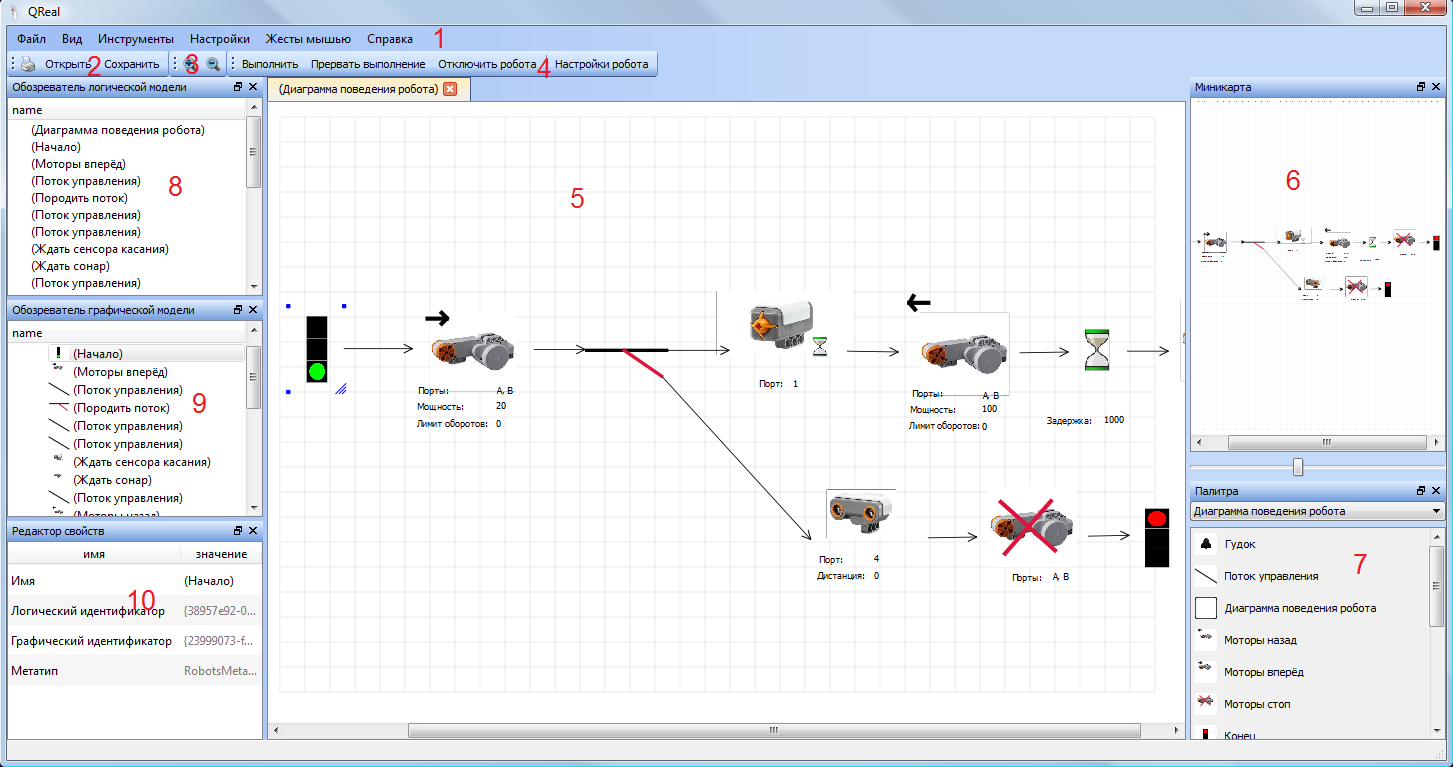
\includegraphics[width=1.00\textwidth]{Interface.png}
    \caption{Главное окно QReal}
    \label{fig:Interface}
  \end{center}
\end{figure}

\pagebreak

\begin{enumerate}
	\item \textbf{Главное меню} --- набор базовых операций и настроек среды. Внимания заслуживает меню "`Инструменты"': 
    \begin{description}
      \item[Выполнить] --- запустить отображаемую в данный момент диаграмму на роботе
      \item[Прервать выполнение] --- остановить выполнение программы, сбросив интерпретатор в начальное состояние
      \item[Отключить робота] --- прервать выполнение программы и послать роботу команды отключения моторов
    \end{description}
  \item \textbf{Панель "`Файл"'} --- позволяет распечатать или сохранить текущую диаграмму, или открыть существующую. При открытии диаграммы надо указывать папку с сохранением --- сохранённая диаграмма сейчас представляет собой набор файлов, разложенных по папкам, и при открытии надо указывать ту папку, которая содержит в себе папку save. Например, чтобы открыть метамодель языка, надо выбрать папку saves/metamodel. Так же сейчас происходит и создание новой диаграммы --- надо нажать "`Открыть"' и в появившемся окне создать новую папку и указать её, или выбрать уже существующую.
  \item \textbf{Панель "`Вид"'} позволяет увеличить или уменьшить изображение на сцене. Это же можно сделать колёсиком мыши
  \item \textbf{Панель "`Интерпретатор"'} содержит команды управления процессом интерпретации диаграммы, соответствующие описанным выше пунктам меню "`Инструменты"'
  \item \textbf{Окно редактора} показывает текущую активную диаграмму, здесь же ведётся её редактирование, здесь же отображается текущий исполняемый блок при исполнении программы
  \item \textbf{Миникарта} --- уменьшенный вид на диаграмму, со слайдером для изменения масштаба изображения
  \item \textbf{Палитра} --- набор доступных блоков, которые можно добавить на диаграмму, перетащив элемент в окно редактора. Связи между элементами добавляются так же, перетаскиванием из палитры. Когда создана новая диаграмма, окно редактора недоступно, нужно перетащить из палитры элемент "`Диаграмма поведения робота"' в окно "`Обозреватель графической модели"' и потом кликуть на нём. После этого в окне редактора откроется вкладка с этой диаграммой и на неё можно будет добавлять элементы. Кроме того, сверху от самой палитры есть выпадающий список загруженных редакторов. Текущая версия имеет два редактора --- метаредактор для просмотра метамодели языка и сам редактор диаграмм поведения роботов, между редакторами можно переключаться с помощью выпадающего списка.
  \item \textbf{Обозреватель логической модели} --- список узлов и связей, присутствующих в программе.
  \item \textbf{Обозреватель графической модели} --- дерево элементов, присутствующих на диаграмме. Одному элементу из логической модели может соответствовать несколько элементов графической модели, каждый элемент на диаграмме --- это образ какого-либо элемента логической модели, у одного элемента может быть несколько образов, эквивалентных с точки зрения логики работы. Интерпретатор диаграмм роботов работает с графической моделью, поэтому логическую модель можно игнорировать.
  \item \textbf{Редактор свойств} --- здесь перечисляются все свойства выделенного в окне редактора элемента, такие, как мощность моторов, порты, длительность операции. Все свойства также можно редактировать непосредственно на диаграмме (двойным кликом по значению свойства), кроме указания типов линий в узлах "`Породить поток"' и "`Цикл"', подробнее об этом ниже.
\end{enumerate}

\section{Доступные блоки}

\begin{center}
	\begin{tabular}{m{0.15\textwidth} | m{0.7\textwidth}}
    {\vspace{10pt}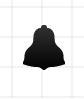
\includegraphics[width=0.15\textwidth]{Beep.png}}          & \textbf{Гудок} --- проиграть на роботе звук с фиксированной частотой. Имеет одно свойство --- ждать завершения проигрывания или сразу же перейти к следующему блоку. Допустимые значения --- true и false\\ \hline
    {\vspace{10pt}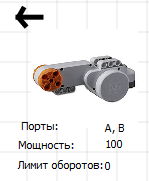
\includegraphics[width=0.15\textwidth]{MotorBackward.png}} & \textbf{Моторы назад} --- включить моторы в режиме реверса по заданным портам с заданной мощностью. Можно также указать лимит оборотов (в градусах), после которых мотор отключится. Порты задаются буквами A, B, C, разделёнными запятыми. Например, на картинке изображена команда включения моторов на портах A и B. \\ \hline
    {\vspace{10pt}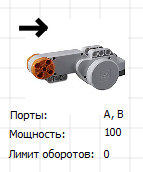
\includegraphics[width=0.15\textwidth]{MotorForward.png}}  & \textbf{Моторы вперёд} --- включить моторы по заданным портам с заданной мощностью. Параметры аналогичны параметрам блока "`моторы назад"', более того, если указать мощность моторов отрицательной, моторы будут включены в режиме реверса. \\  \hline
    {\vspace{10pt}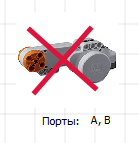
\includegraphics[width=0.15\textwidth]{MotorStop.png}}     & \textbf{Моторы стоп} --- выключить моторы по заданным портам. \\ \hline
    {\vspace{10pt}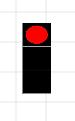
\includegraphics[width=0.10\textwidth]{End.png}}           & \textbf{Конец} --- конец выполнения программы. Если программа состоит из нескольких параллельных нитей, достижение этого блока заканчивает текущую нить. \\ \hline
    {\vspace{10pt}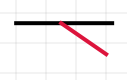
\includegraphics[width=0.15\textwidth]{Fork.png}}          & \textbf{Породить поток} --- разделить выполнение программы на два потока, которые будут выполняться псевдопараллельно. Так, например, можно одновременно ждать срабатывания сенсора или истечения временного интервала. Узел должен иметь две исходящие, одна из которых помечена словом "`другой"' (то есть, это слово надо вписать в поле Guard в редакторе свойств, предварительно выделив нужную связь). \\ \hline
	\end{tabular}
\end{center}
    
\begin{center}
	\begin{tabular}{m{0.2\textwidth} | m{0.7\textwidth}}
    {\vspace{10pt}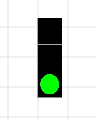
\includegraphics[width=0.15\textwidth]{Begin.png}}         & \textbf{Начало} --- начальная точка выполнения программы, должна быть на диаграмме одна, с неё начинается процесс интерпретации, здесь же устанавливается соединение с роботом и выполняется его инициализация, так что на этом блоке интерпретатор может задержаться на некоторое время. \\ \hline
    {\vspace{10pt}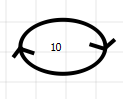
\includegraphics[width=0.15\textwidth]{Loop.png}}          & \textbf{Цикл} --- блок, организующий выполнение последовательности операторов несколько раз (количество повторений указывается единственным параметром). Должен иметь две исходящие дуги, одна из исходящих дуг должна быть помечена словом "`итерация"' (то есть свойство Guard в редакторе свойств должно быть установлено в "`итерация"'). Работает он так: каждое посещение этого блока в процессе работы программы уменьшает счётчик на 1, счётчик инициализируется значением параметра (по умолчанию 10). Если счётчик больше 0, происходит переход по связи "`итерация"', если нет --- по непомеченной исходящей связи. Бесконечные циклы можно организовать без использования специальных блоков, просто соединив связью конец цикла с началом. \\ \hline
    {\vspace{10pt}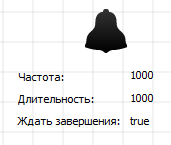
\includegraphics[width=0.15\textwidth]{PlayTone.png}}      & \textbf{Играть звук} --- играть звук с заданной частотой и длительностью. Аналогичен блоку "`Гудок"', но позволяет задавать параметры звука. Имеет параметр, определяющий, ждать завершения проигрывания или сразу же перейти к следующему блоку. \\ \hline
    {\vspace{10pt}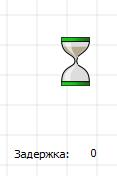
\includegraphics[width=0.15\textwidth]{Delay.png}}         & \textbf{Таймер} --- ждать заданное количество времени, в миллисекундах. \\ \hline
    {\vspace{10pt}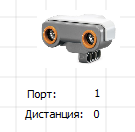
\includegraphics[width=0.15\textwidth]{WaitForSonar.png}}  & \textbf{Ждать сонар} --- ждать, пока расстояние, возвращаемое ультразвуковым сенсором, не будет меньше указанного в параметре (в сантиметрах, от 0 до 255). Также параметром указывается порт, на котором расположен сенсор, допустимые значения: 1, 2, 3, 4. \\ \hline
    {\vspace{10pt}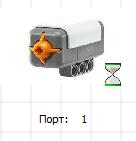
\includegraphics[width=0.15\textwidth]{WaitForTouch.png}}  & \textbf{Ждать сенсор касания} --- ждать, пока не сработает сенсор касания. Также параметром указывается порт, на котором расположен сенсор, допустимые значения: 1, 2, 3, 4. \\ \hline
	\end{tabular}
\end{center}

\end{document}